
\documentclass{article}
\usepackage{amsmath, amsthm, graphicx}
\usepackage[accepted]{icml2018}
% \usepackage{lastpage}
% \fancyfoot[C]{Page \thepage\ of \pageref{LastPage}}
\usepackage{url}
\usepackage{fancyhdr}
\pagestyle{fancy}
\fancyhf{}
\fancyhead[R]{\thepage}

\icmltitlerunning{A Brief History of Deep Learning Methodologies for Solving Combinatorial Optimization Problems}

\begin{document}
\twocolumn[
\icmltitle{A Brief History of Deep Learning Methodologies for Solving Combinatorial Optimization Problems}

\begin{icmlauthorlist}
\icmlauthor{Rahul Thapa}{vu}
\end{icmlauthorlist}

\icmlaffiliation{vu}{Department of Computing Sciences, Villanova University,
Villanova, PA}

\icmlcorrespondingauthor{Rahul Thapa}{rthapa@villanova.edu}

% You may provide any keywords that you
% find helpful for describing your paper; these are used to populate
% the "keywords" metadata in the PDF but will not be shown in the document
\icmlkeywords{Hopfield Neural Network, Self Organizing Feature Maps, Travelling Salesman problem (TSP), Deep Reinforcement Learning, Pointer Network, Deep Learning, Graph Convolutional Network (GCN), Deep Q-Learning (DQN)}

\vskip 0.3in
]

%\printAffiliationsAndNotice{}  

\begin{abstract}
Combinatorial Optimization Problems (COPs) involve finding an optimal solution within a finite set of possible solutions. Generally, the solution set is large and hence, is not practical to be solved through exhaustive search. Researchers have proposed many exact as well as approximate algorithms for solving COPs. However, such approaches are not very scalable because most of the COPs are NP-hard. In this survey, we present various deep learning methodologies used to solve discrete COPs and compare their network architectures and results. We begin with an introduction of two very popular neural network-based approaches called Hopfield Network and Self Organizing Feature Maps to solve COPs. As the core focus of our survey, we present extensive research done on solving COPs using deep learning within the past ten years. We discuss both supervised as well as unsupervised learning methodologies. Finally, we describe some current areas of research as well as challenges within this field. 
\end{abstract}

\section{Introduction}
Combinatorial optimization is a topic that consists of finding an optimal object from a finite set of objects. The set of possible solutions is discrete and generally defined by a set of restrictions. It is often hard to solve such problems because the solution set is too large for exhaustive search. Combinatorial optimization has important real-world applications such as optimizing the supply chain, determining the optimal way to deliver packages, allocating jobs to people in the best possible way, developing the best airline network of spokes and destinations. Some of the most popular COPs are Knapsack problem, Travelling Salesman Problems (TSP), Maximum Vertex Cover, and Satisfiability (SAT). In this paper, we discuss deep learning methodologies used to solve varieties of these problems. However, a lot of these approaches are targeted towards solving one particular COP i.e. TSP. Therefore, we provide a brief introduction along with the exact and approximate methods used to solve it. 

\begin{figure}
    \centering{
    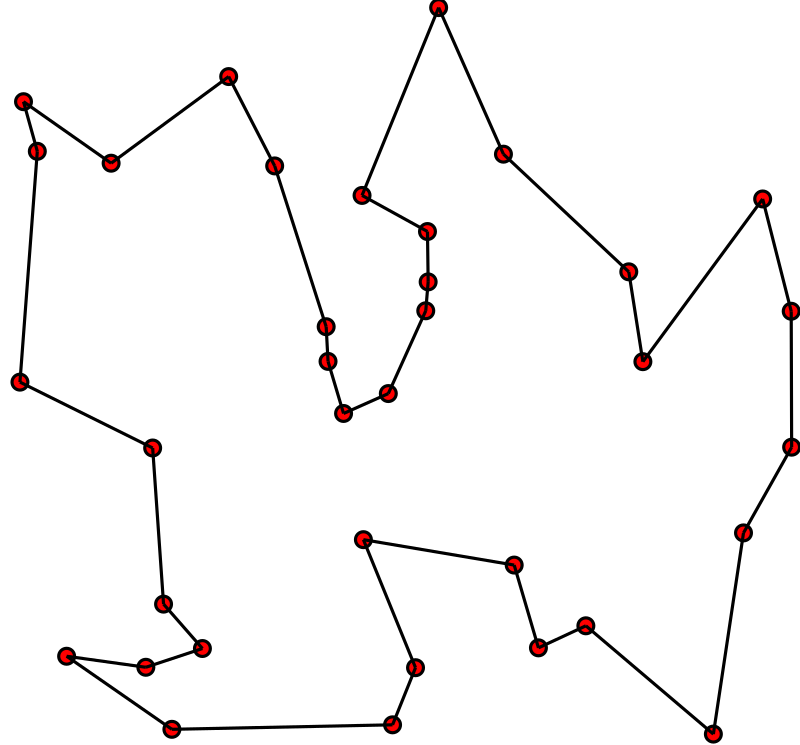
\includegraphics[scale=0.2]{images/tsp.png}}
    \caption{An optimal solution of a travelling salesman problem. The black line shows the shortest possible path that connects every red dot. Figure adapted from \cite{wikipedia_2020}}
    \label{fig:tsp}
\end{figure}

The origin of TSP dates back to the 1800s, however, its mathematical forms were initiated in 1930 \cite{sarwar2012critical}. In this problem, given a list of cities, one must find the shortest possible route that visits a set of cities all only once and returns to the original city, as shown in Figure \ref{fig:tsp}. Some of the applications of TSP are delivering packages in a most cost-efficient way, drilling printed circuits, and picking order in a warehouse \cite{applegate2006traveling, la2012comparison, junger1994provably}. Even though the problem sounds fairly easy, it is not so easy to solve as it falls under NP-hard problems, even in two-dimensional Euclidean case \cite{padberg1991branch, bello2016neural}. 

Many exact and approximate algorithms have been proposed to solve TSP as surveyed in \cite{laporte1992traveling}. The exact dynamic programming algorithm for TSP has a time complexity of $\theta(2^nn^2$). Some of the methods included in \cite{laporte1992traveling} are the branch-and-bound method, integer linear programming, and shortest spanning arborescence bound method. Because of exponential time complexity, it is not feasible to implement the exact algorithm for practical application. Christofides proposed an O(n$^3$) heuristic algorithm that involves computing a shortest spanning tree and a minimum cost perfect matching \cite{christofides1976worst, bello2016neural, laporte1992traveling}. Similarly, Lin-Kernighan-Helsgaun heuristic, which was extended from Lin-Kernighan heuristic, is a popular approximate search heuristic which can solve instances with hundreds of nodes \cite{bello2016neural, helsgaun2000effective, lin1973effective}. This approach yields state-of-the-art results for symmetric TSP. Voudouris et al. \cite{voudouris1999guided} used Guided Local Search (GLS) and Fast Local Search (FLS). GLS lied on top of local search heuristic and it was combined with the neighborhood reduction scheme of FLS.

It has been over four decades since researchers started using artificial neural networks to find an optimal solution to TSP \cite{smith1999neural}. Hopfield and Tank designed one of the first neural networks to find an optimal path to TSP \cite{hopfield1985neural}. They quantitatively demonstrated the computational power and speed of analog networks of neurons. However, \cite{wilson1988stability} pointed out that this network was not very stable and reported unsatisfactory results even with a slight modification to the original algorithm. Many other researchers have expanded on this network \cite{aiyer1990theoretical}. One of the most recent works on this network is done by \cite{sarwar2012critical} in which the authors compare the Hopfield Network with the heuristic algorithm. 

Another main approach for solving TSP is by using Kohonen's Self-Organizing Feature Map \cite{kohonen1982self}. A vast majority of these approaches are based on elastic net method \cite{durbin1987analogue} in which Kohenen's principles of self-organization are combined with the concept of the "elastic band" containing circular rings of neurons \cite{durbin1987analogue, smith1999neural}. Self-organizing nets have also been applied to solve other problems such as vehicle routing problem \cite{vakhutinsky1994solving}. An overview of a wide range of its applications can be found in \cite{kohonen1990self}. 

\cite{sarwar2012critical} showed that neural networks were still not able to yield comparable results to exact methods. Some of the reasons for a mediocre success of this field can be attributed to lack of powerful hardware resources and powerful neural network methodologies. This particular field remained stagnant for about a decade after 2000 \cite{bello2016neural}. However, with the rejuvenation of deep learning \cite{lecun2015deep}, researchers once again began applying artificial neural networks to solving COPs. This can be attributed to the advancement of some crucial deep learning methodologies such as sequence-to-sequence model \cite{sutskever2014sequence}, attention mechanism \cite{bahdanau2014neural}, graph convolutional network (GCN) \cite{kipf2016semi}, and deep reinforcement learning (DRL) \cite{mnih2015human}. One of the popular works is the Pointer Network introduced by \cite{vinyals2015pointer}. This network utilizes a recurrent neural network trained in a supervised manner to predict the sequence of visited cities. A simplified version of the Pointer Network for solving vehicle routing problems is presented in \cite{nazari2018reinforcement}. \cite{bello2016neural} significantly outperformed this supervised learning approach by using reinforcement learning and neural networks on a 2D Euclidean graphs. Similarly, \cite{khalil2017learning} solved optimization problems over graphs using graph embedding and deep Q-learning (DQN) algorithms \cite{mnih2015human}. \cite{li2018combinatorial} presented a related work but differed in some key aspects. For example, \cite{li2018combinatorial} used supervised learning instead of RL and GCN as their predictive model.   

The remainder of this paper is organized into four sections. Section II discusses the use of neural networks to solve combinatorial optimization problems. This part specifically focuses on research done on this domain before 2000. Two main approaches we discuss under this section are Hopfield Neural Network and Self-Organizing Feature Maps based approaches. 
%Section III introduces a few deep learning networks that are crucial to understanding the subsequent work. 
Section III focuses on the application of Deep Neural Networks to solving COPs. The majority of the paper concentrate on this section. Section IV discusses some current challenges in this field along with most recent works proposed to tackle those challenges. Finally, section V concludes the survey with a brief summary.


\section{Neural Network based Approaches}
Even though this paper is a survey on Deep Learning methodologies for solving COPs, it is crucial to understand how researchers started using artificial neural nets to solving COPs. In this section, we briefly discuss some famous neural network based approaches such as Hopfield Network and Self-Organizing Feature Maps. A lot of work done before the 2000s in this domain were influenced by or extended from these networks. 

\subsection{Hopfield Neural Network}
Hopfield network was modeled initially to enable a content addressable memory \cite{smith1999neural} by John Hopfield in his 1982 seminal paper \cite{hopfield1982neural}. He introduced a new way of modeling a system of neurons capable of performing computational tasks. In 1985, John Hopfield and David Tank extended the Hopfield Neural Network model to solve optimization problems \cite{hopfield1985neural}. They selected weights and external inputs of their neural network that approximately represented the function to be minimized and the desired states of the problem. For rapid and powerful solution techniques, they combined the analog nature of the neurons and the parallel processing of the updating procedure. The object function and energy function of the network were made equivalent which needed to be minimized i.e. the lowest energy state or stable states corresponds to the best path. The constraint of the optimization was included as penalty terms in the energy function. One pitfall of this approach was that these stable states might not correspond to optimal solutions, as the energy function might get stuck in one of many poor local minimums \cite{smith1999neural}.

\begin{figure}
    \centering{
    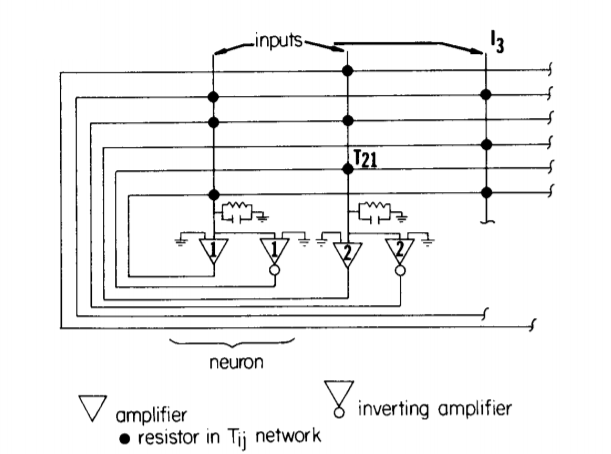
\includegraphics[scale=0.7]{images/hopfield-network.png}}
    \caption{A simple analog representation of Hopfield and Tank Network that can solve optimization problems. The output of any neuron can potentially be connected to the input of any other neuron. Black circles represent resistive connections between inputs and outputs. Figure adapted from \cite{hopfield1985neural}.}
    \label{fig:hopfield-network}
\end{figure}

Hopfield and Tank's network was successfully applied to many optimization problems, however, their results for TSP gained most interest among the research community. They simulated a 10-city problem with 100 neurons \cite{hopfield1982neural}. They chose the locations of the cities at random on the interior of a two-dimensional unit square. They claimed that they were able to find the appropriate general size of the parameters easily and that they used anecdotal exploration of parameter values to find a good operating point. However, they acknowledged that these points may not be optimal. They also acknowledged that the sensitivity of the results was due to the parameter settings of the network. For the 10 city problem, their model converged 16 out of 20 random starts to a valid tour. About 50\% of the trials produced one of the two known shortest tours \cite{hopfield1985neural, smith1999neural}. However, their model did not do so great on larger sized inputs. For example, for a 30-city and 900 neurons problem, their results were fragmentary. They reported that the parameter choice appeared to be a more delicate issue for a larger network. 

\subsubsection{Limitations of Hopfield Neural Network}
One of the most popular works that raised doubt on the reliability and validity of Hopfield and Tank's approach to solving COPs was \cite{wilson1988stability} by Wilson and Pawley. While trying to imitate \cite{hopfield1985neural} approach to find the parameter settings for a larger problem size, they realized that the model did not converge to any valid solution. Even in a similar 10-city problem as proposed in \cite{hopfield1985neural}, they were only able to converge 15 of the 100 random starts to valid tours which were not much better than random choices. Many of them got stuck into local minima. This result was much worse than what Hopfield and Tank reported \cite{wilson1988stability}. After trying some modifications such as change in parameter selection and increasing the value of the distance from a city to itself and not being able to get a significant improvement, they hypothesized that the root of the problem could be in the method, and not the operating point \cite{smith1999neural}. There are some other works \cite{kamgar1992dynamical}, that have raised doubts on the stability of Hopfield and Tank's approach. \cite{lister1993annealing} questioned the necessity of an energy function with a high degree of ultrametricity.

\subsubsection{Hopfield Network Extensions}
Despite various criticism of Hopfield Networks in solving COPs, various extension of this network had been proposed in solving TSP \cite{den1988traveling, gee1995limitations, yao1988alternative, lin1994impact}. Extension of Hopfield Neural Networks involved two changes: First, modifying the energy function to eliminate the trade-off problems between valid and good solutions. Second, searching for ways to optimally select the penalty parameters while keeping the original energy function \cite{smith1999neural}. 

In \cite{den1988traveling}, the authors formulated a new TSP objective function which requires the setting of only one parameter to balance the importance of tour length and feasibility. This parameter is easy to determine from city distance. They also designed a new algorithm called Mean Field (MF) to handle the constraint that each city exists at one and only one tour position. This modification helped them find consistent valid and near-optimal solutions for a 30 city problem.

Another research around the same time \cite{den1988traveling} used a modified penalty function to overcome the difficulty of consistently producing valid tours \cite{yao1988alternative}. With this modified network, they were able to generate 21/21 valid tours. They also formulated a fixed-parameter network whose connection matrix did not depend on problem data and could be fixed at hardware fabrication time for TSP.

The most comprehensive study of various modifications in the energy function of the original Hopfield and Tank's model was done by \cite{lin1994impact}. They evaluated six different variations to the energy function. One of the popular approaches that they included was Aiyer energy function\cite{aiyer1990theoretical}. Aiyer et al. utilized the eigenvalues of weights to introduce adjusting constantly into the energy function and corrected the landing error in the valid sequence. Out of all six approaches, Aiyer energy function was able to converge to a valid solution largest number of times. On 10-city topology benchmarks, the convergence percentage of Aiyer energy function for most benchmarks was above 90\%.


\subsection{Self-Organizing Feature Map}
The self-organizing feature map (SOFM) is an unsupervised neural network that learns from the pattern of the input data and organizes itself based on that \cite{kohonen1982self}. It differs from Hopfield Network in that it does not contain preset weights and does not require supervision to guide the network. In such a network, first, the input patterns of arbitrary dimensionality are converted into one or two-dimensional array of neurons as shown in Figure \ref{fig:self-organizing-map}. Each component in the input vector x is connected to each of the neurons, and the weight $W_{ij}$ transmits the input $x_j$ toward the $j^{th}$ neuron of the feature map \cite{smith1999neural}. Learning is then achieved via adaptation of the weights connecting the input patterns to the array of neurons. The learning process comprises two stages: a competitive stage and an adaptive stage. On a competitive stage, a neuron that is closest to the input data called winning neuron \cite{smith1999neural} is identified. On the adaptive stage, the weights of the winning neuron and its surrounding neurons are adjusted \cite{kohonen1982self}.   
\begin{figure}
    \centering
    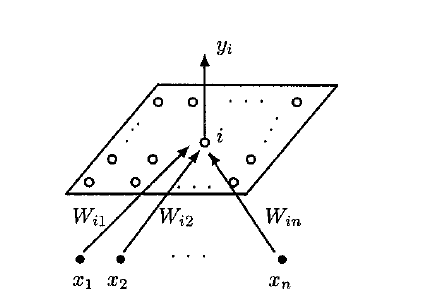
\includegraphics{images/self-organizing-map.png}
    \caption{Mapping features of input vector x onto a two-dimensional array of neurons in Kohonen's SOFM. Adapted from \cite{smith1999neural}.}
    \label{fig:self-organizing-map}
\end{figure}

\subsubsection{Limitations of Self-Organizing Neural Network}
\cite{bishop1997gtm} discussed some significant limitations of the Self-Organizing Map. They claimed that the algorithm was at a disadvantage because it was not derived by optimizing an objective function. Similarly, in such maps, the neighborhood-preservation was also not guaranteed. Furthermore, the choice of how the neighborhood function should shrink over time was arbitrary during training.

\subsubsection{Self-Organizing Feature Map Extensions}
One of the most popular ways the principles of self-organization maps were applied to solving TSP was by merging it with the elastic net method. The elastic net was first proposed by Durbin and Willshaw in \cite{durbin1987analogue} to solve TSP. The algorithm starts with k points, greater than the number of cities, lying on a hypothetical "elastic band". When the nodes are moved, the "elastic band" stretches in such a way that minimizes the energy function \cite{smith1999neural, durbin1987analogue}. Sometimes, this method is considered analogous to the gradient descent of the energy function. Durbin and Willshaw were able to achieve state-of-the-art solutions \cite{lin1973effective} at the time of its publication. Their solution was 19\% better than the Hopfield and Tank's best solution in terms of solution quality \cite{smith1999neural}. However, the limitation of this approach is that it can be applied only to Euclidean TSPs and related problems.

A Self-Organization map approach to solving TSP, which is a very similar approach to the elastic method, was presented by \cite{fort1988solving} where they used a one-dimensional circular array of neurons and mapped it onto the TSP cities such that two neighboring points on the array were also neighbors in distance \cite{smith1999neural}. There are some major differences, but the basic idea is the same, which even Fort agreed to in \cite{fort1988solving}. However, the result that Fort obtained in a similar experiment done by \cite{durbin1987analogue} was not as good.

Another group of researchers began experimenting by combining elastic net and SOFM to solve the TSP. One of the first approaches was by \cite{angeniol1988self}. They had a set of nodes joined together in a continuous ring. The nodes were free to move in a Euclidean plane iteratively until a complete tour was obtained when every city catches a node in the ring \cite{smith1999neural}. They also included rules to create and delete nodes in their network. In a similar set of TSPs used by Hopfield and Tank \cite{hopfield1985neural}, Ang\'eniol et al. obtained a result that was comparable to the best result of \cite{durbin1987analogue}.

An alternative to the approach suggested by \cite{angeniol1988self} is \cite{burke1992guilty}. Burke and Damany eliminated the need for the node creation and deletion rules. Their network is called the guilty net in which the number of nodes is equal to the number of cities. This network was inspired by the idea of conscience introduced in \cite{desieno1988adding}. This ensured the feasibility of the TSP tour as a minimum requirement, even if the network terminated prematurely \cite{smith1999neural}. The results presented in \cite{burke1992guilty} for TSP problems are poorer than the elastic net method. However, the authors noted that the number of iterations required was substantially lower. Burke later extended the guilty network called the vigilant net \cite{burke1994neural}. This network was inspired by the vigilance of the adaptive resonance networks \cite{carpenter1987art}.
 
% \section{Some Core Deep Learning Approaches}
% With the advent of deep learning, a significant impact has been made in various fields of machine learning such as object detection, speech recognition, and language translation \cite{lecun2015deep}. The property of deep learning that makes it so influential is the deep neural networks that can automatically find compact low-dimensional representations or features of high-dimensional data. Through crafting inductive biases into neural network architectures, particularly that of hierarchical representations, machine learning practitioners have made effective progress in addressing the curse of dimensionality \cite{bengio2013representation}. One field that was stagnant for over a decade, that has been rejuvenated by the advent of deep learning is solving COPs using neural network. Before diving into various deep learning methodologies used to solve the COPs, it is essential to understand some important networks that use deep learning. A lot of the research works done in this domain uses these approaches. Therefore, having a basic understanding of these deep learning frameworks that will be used in subsequent work of solving COPs is essential. 

% \subsection{Sequence-to-Sequence Learning}
% Sequence to Sequence Models can be used for problem domain in which mapping from one sequence to another sequence is required \cite{sutskever2014sequence, vinyals2015pointer, luong2015effective}. A multilayered Recurrent Neural Network (RNN) such as Long Short-Term Memory (LSTM), which is called an encoder, is used to map the input sequence to a vector of fixed dimensionality. Another Deep LSTM, called decoder, is then used to decode the target sequence from the vector %as shown in Figure \ref{fig:seq-to-seq}
% . Such a model has had a significant contribution to the neural machine translation. Bahdanau et al. extended on this encoder and decoder network by employing another neural network called attention mechanism \cite{bahdanau2014neural}.

% % \begin{figure}
% %     \centering{
% %     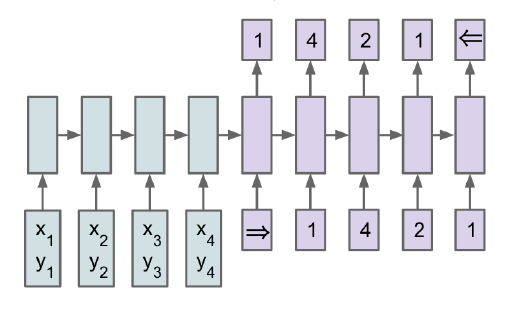
\includegraphics[scale=0.85]{seq-to-seq.png}}
% %     \caption{Sequence-to-Sequence - The blue color boxes represent RNN that processes the input sequence and creates a code vector which is used to generate the output sequence using another RNN represented by purple boxes. The input and output dimentionality are same during training and inference and is fixed by the dimentionality of the problem. Figure adapted from \cite{vinyals2015pointer}.}
% %     \label{fig:seq-to-seq}
% % \end{figure}

% The content-based attention mechanism allowed them to propagate extra contextual information from the input. By allowing the decoder network to focus on the important locations of the source sequence and use the relevant information, they were able to produce better output sequences. A drawback of these methods is that they require the size of the output dictionary to be fixed a priori \cite{vinyals2015pointer}. Due to this reason, such methods can not be directly applied to combinatorial problems as in such problems, the size of the output dictionary depends on the length of the input sequence.

% \subsection{Graph Embedding}
% Graph embedding is the process of transforming nodes, edges, and their features in a graph into a vector space. The goal is to transform the graph into a lower dimension while still preserving the properties of graph structure and information in it. There are various approach to graph embedding such as DeepWalk \cite{perozzi2014deepwalk}, Node2vec \cite{grover2016node2vec}, Graph2vec \cite{narayanan2017graph2vec}, Structural Deep Network embedding \cite{wang2016structural}, structure2vec \cite{dai2016discriminative}. In this paper, we will only discuss structure2vec.

% Structure2vec is an efficient and scalable approach for structured data representation based on the idea of embedding latent variable models into feature spaces and learning such feature spaces using discriminative information. This model was created to scale up kernel methods for structured data to millions of data points, and allowing the kernel to learn the feature representation from label information. Structure2vec models each structured data point as a latent variable model, then embed the graphical model into feature space \cite{scholkopf2002learning}. After that, the inner product in the embedding space is used to define kernels. Dai et al. \cite{dai2016discriminative} claim that structure2vec extracts features by performing a sequence of function mappings in a way similar to graphical model inference procedures, such as mean field and belief propagation.  

% \subsection{Graph Convolutional Network (GCN)}
% GCNs are powerful neural network architecture for machine learning on the graph. Given a graph $G = (V, E)$, a GCN takes an input feature matrix N $\times$ F where N is the number of nodes and F is the number of input features for each node. It also takes N $\times$ N matrix representation of the graph structure such as the adjacency matrix of G \cite{thomas_kipf}. A hidden layer in the GCN can then be written as $H^i = f(H^{i-1}, A)$, where $H$ is the feature matrix and f is the propagation \cite{thomas_kipf}. Each layer $H^i$ corresponds to an N $\times$ $F^i$ feature matrix where each row is a feature representation of a node. At each layer, these features are aggregated to form the next layer's features using the propagation rule $f$. The features become increasingly more abstract at each consecutive layer. In this framework, variants of GCN differ mostly in the propagation rule $f$ \cite{thomas_kipf}.   

% \subsection{Deep Reinforcement Learning}
% Reinforcement learning (RL) is a principled mathematical framework for experience-driven autonomous learning \cite{sutton2018reinforcement}. However, two big problems with approaches utilizing RL were that they lacked scalability and were inherently limited to fairly low-dimensional problems \cite{arulkumaran2017brief}. With the rise of deep learning, relying on the powerful function approximation and representation learning properties of deep neural networks has provided researches with new tools to overcome these problems. Therefore, the use of deep learning algorithms within RL has defined the field of deep reinforcement learning (DRL). DRL can scale to previously intractable decision-making problems, i.e. settings with high-dimensional state and action space \cite{arulkumaran2017brief}. In general, DRL is based on training deep neural networks to approximate the optimal policy $\pi^*$, and/or optimal value function $V^*$, $Q^*$, and $A^*$.

% In this paper, we talk about deep learning frameworks that use deep Q-learning (DQN) \cite{mnih_2015_human}, which is a value-function based DRL algorithm. In short, it is a combination of Q learning and deep neural networks. The simple idea is to replace the Q learning table with a neural network that approximates Q values and denoted as Q(s, a; $\theta$), where s, a are state action pair and $\theta$ represents the trainable parameters of the deep neural network.

% Now that we have covered the basics, we can dive into their application for combinatorial optimization tasks.

\section{Deep Learning Methodologies}
With the advent of deep learning, a significant impact has been made in various fields of machine learning such as object detection, speech recognition, and language translation \cite{lecun2015deep}. The property of deep learning that makes it so influential is the deep neural networks that can automatically find compact low-dimensional representations or features of high-dimensional data. Through crafting inductive biases into neural network architectures, particularly that of hierarchical representations, machine learning practitioners have made effective progress in addressing the curse of dimensionality \cite{bengio2013representation}. One field that was stagnant for over a decade, that has been rejuvenated by the advent of deep learning is solving COPs using artificial neural network. This section describes some popular supervised as well as unsupervised learning-based approaches in solving COPs.  
% This section occupies the majority of the paper. We will specifically focus on the research conducted in solving COPs using Deep Learning methodologies after 2010. Deep Learning started to come to the mainstream again around that time. Like we mentioned previously, this deep learning boom urged researchers to turn their focus back to solving a combinatorial optimization problem using artificial neural networks | the field that was widely abandoned after 2000. 

\subsection{Supervised Learning}
One of the first attempts to tackle the COPs using deep learning methodology was proposed by \cite{vinyals2015pointer}. They introduced the concept of pointer network, which was inspired by sequence-to-sequence models \cite{sutskever2014sequence}. The Sequence-to-sequence learning method requires the size of the output dictionary to be fixed a priori \cite{vinyals2015pointer}. However, in COPs, the output sequence length is determined by the source sequence. Therefore, Vinyals et al. had to modify the sequence-to-sequence model to make it invariant to the length of the encoder sequence. They modified the attention mechanism of \cite{bahdanau2014neural} to create pointers to input elements as shown in Figure \ref{fig:ptr-net}.

\begin{figure}
    \centering{
    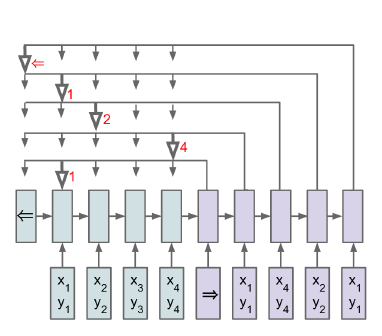
\includegraphics[scale=1]{images/ptr-net.png}}
    \caption{Pointer Network - The encoder RNN network, represented by blue boxes, covers the input sequence to a code that is then fed to the generating network represented by purple boxes. The output of generating network is a vector that modulates a content-based attention mechanism over input. Figure adapted from \cite{vinyals2015pointer}.}
    \label{fig:ptr-net}
\end{figure}

Given a training pair $(P, C^P)$, the traditional sequence-to-sequence model computes the conditional probability $p(C^p|P;\theta)$ as

\begin{equation}
    p(C^P|P;\theta) = \prod_{i=1}^{m(P)} p(C_i|C_1,...,C_{i-1}, P;\theta)
    \label{eq:1}
\end{equation}

Here, $P = \{P_1,..., P_n\}$ is a sequence of n vectors and $C^P = \{C_1,..., C_{m(P)}\}$ is a sequence of $m(P)$ indices. An RNN with parameters $\theta$ is used to estimated the terms of the probability. This model uses softmax distribution over a fixed sized output dictionary to compute $p(C_i|C_1,...C_{i-1},P)$ in Equation \ref{eq:1} which can not be used for COPs because the size of the output dictionary is equal to the length of the input sequence. Therefore, Vinyals et al. used attention mechanism to model $p(C_i|C_1,...C_{i-1},P)$ as follows:

\begin{align*}
    u^i_j &= v^T \text{tanh}(W_1e_j + W_2d_i) \hspace{0.2cm} j \in (1,...,n) \\
    p(C_i|C_1,...,C_{i-1},P) &= \text{softmax}(u^i)
    \label{eq:2}
\end{align*}

Here, $v, W_1$ and $W_2$ are learnable parameters of the output model. Softmax normalizes the vector $u^i$ to be the attention mask over the inputs i.e. pointers to the input elements. Their approach was specifically designed for problems whose outputs are discrete and correspond to the positions in the input. 

Vinyals et al. used the same model architecture to perform experiments on 3 problem sets: Convex Hall \cite{graham1972efficient, jarvis1973identification}, Delaunay Triangulation \cite{rebay1993efficient}, and TSP. All their models used a single layer LSTM trained with stochastic gradient descent. They used the convex hull as a baseline to understand the deficiencies of the traditional sequence-to-sequence model and build their pointer network. They checked the performance of their model for a convex hull experiment based on accuracy and area covered of the true convex hull. They noted that the area coverage achieved with the Ptr-Net was close to 100\%. They observed that the order in which the inputs are presented matter during inference as it affected the performance when there was not attention mechanism. However, the attention mechanism allowed their decoder to look at the whole input at any time and hence, overcome this problem. They observed that the attention was pointing at the correct answer on the input side. The major contribution of this experiment was showing that their model had the key advantage of being inherently variable length. A single model trained on a variety of lengths performed quite well on all lengths it was trained on. They even noticed that their model even extrapolated to lengths that it had never seen before. They noted their result for n=500 which gave them a satisfactory result, while other models with LSTM or LSTM with attention could not even be used for any given input size that they had not been trained on. 

For the experiment on TSP, they considered planner symmetric TSPs. Since their algorithm for Ptr-Net implemented an $O(n^2)$ algorithm, initially, they were not very clear if their model would be able to learn solely from data. To make sure that the model would not output invalid tours, they used beam search procedure for input size n $>$ 20. As it is feasible to generate exact solutions for relatively small-sized TSP, they used three different algorithms A1, A2, and A3 to generate approximate solutions for large-sized TSP. They trained their Ptr-Net model on optimal data with 5 to 20 cities to see if they could generalize for larger values of n. They noted that their model performed pretty good for $n = 25$ and reasonably good for $n = 30$. However, their model broke for values higher than 40. 

\cite{li2018combinatorial} is another prominent work to solve COPs that harnesses graph property of some COPs such as TSP. They used GCN to predict the likelihood, for each vertex, of whether this vertex was part of the optimal solution. Li et al. extended from \cite{khalil2017learning}, which was one of the first approaches to solving COPs in terms of a graph. We will discuss this in the next subsection. The approach outlined in Li et al. differs from the one proposed by Khalil et al. in 3 key respects.

First, they did not use reinforcement learning because they considered it a particularly challenging method. Rather, they used supervised learning and showed that they could achieve strong performance and generalization and could benefit from well-understood and reliable solvers. Second, they used GCN as opposed to Deep Q-learning (DQN) network with graph embedding in \cite{khalil2017learning}. Finally, they designed and trained the network to synthesize a diverse set of solutions at once which was key to their approach and allowed them to rapidly explore the solution space. 

Li et al. focused on four canonical NP-hard problems: Maximal Independent Set (MIS), Minimum Vertex Cover (MVC), Maximal Clique (MC), and Satisfiability (SAT). One key property of these problems is that they can be reduced to each other \cite{karp1972reducibility} in polynomial time. For example, MVC, MC, and SAT problems can all be represented as instances of the MIS problem. Therefore, this paper primarily focused on the MIS problem, although, the basic structure of the approach was general. 

\begin{figure*}
    \centering{
    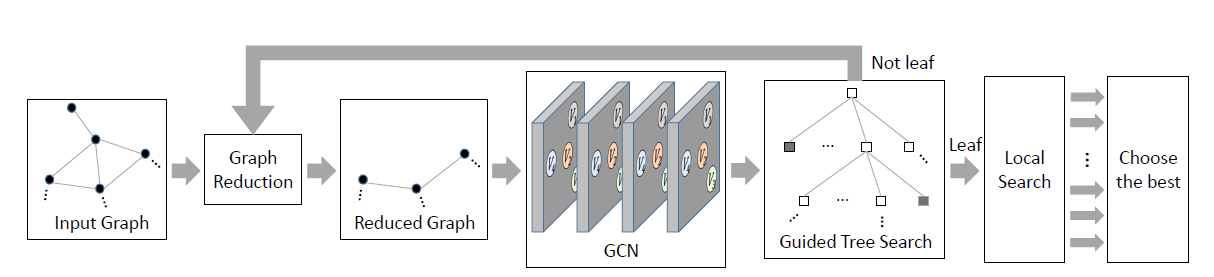
\includegraphics[scale=0.65]{images/gcn.png}}
    \caption{The Deep learning architecture of the algorithm defined in Li et. al. Graph Convolutional Network is used to generate the multiple probability maps which are used to iteratively label the vertices until all vertices are labeled. Labeling is generated by the guided tree search and refined by rapid local search. Figure adapted from \cite{li2018combinatorial}.}
    \label{fig:GCN}
\end{figure*}

In Figure \ref{fig:GCN}, we can see that there were 4 major parts of their network architecture: graph reduction, GCN, tree search, and local search. First was the graph reduction step in which they rapidly reduced a graph into a smaller one while preserving the size of the optimal MIS. This accelerated computation by focusing computation on the complex part of the graph \cite{li2018combinatorial}.

The second part was the graph convolutional network \cite{karp1972reducibility} $f$ which can perform dense prediction over a graph with pairwise edges. The $f$ generated probability maps from the reduced graph, which encoded the likelihood of each vertex being in the optimal solution. The reason that they did not generate a binary vector, 0 and 1, but a real-valued vector in $[0, 1]^N$ was because simply rounding the real values to 0 or 1 might violate the independence constraints. The probability maps were used to iteratively label the vertices until all vertices were labeled. In this setup, $f$ was used as a heuristic function for a greedy search algorithm for MIS. Given a graph $G$, the search algorithm labeled a batch of vertices with 1 or 0 recursively. First, they sorted all the vertices in descending order based on $f(G)$ and iterated over the sorted list in order and labeled each vertex as 1 and its neighbor as 0. This process stops when the next vertex in the sorted list is already labeled as 0. They removed all the labeled vertices and the incident edges from $G$ and obtained a residual graph. This residual graph was fed as an input to $f$ which gave a new likelihood map. This process was repeated iteratively. 

The third part was the tree search. Li et. al. noted that just graph reduction and GCN could confuse the network when there were multiple optimal solutions for the same graph. In other words, the solution space is multimodal and many different modes may be encountered during training \cite{li2018combinatorial}. To enable the network to differentiate between different modes, they extended the structure of $f$ to generate multiple probability maps. To generate diverse high-quality probability maps, they used the hindsight loss \cite{li2018combinatorial}. Producing multiple diverse probability maps also helped them to explore multiple solutions with each run of $f$. The basic idea of a tree search algorithm is that one maintains a queue of incomplete solutions and randomly chooses one of them to expand in each step. When they expanded an incomplete solution, they used $M$ probability maps to spawn $M$ new more complete solutions, which were added to the queue. This process is akin to the breadth-first search algorithm, rather than depth-for search, which they noted, did not yield diverse solutions \cite{li2018combinatorial}. To this end, the expanded tree nodes were kept in a queue and one was selected at random in each iteration for expansion.  

The last step was a local search which helped them refine the candidate solutions produced by tree search. They specifically used a 2-improvement local search algorithm \cite{andrade2012fast, feo1994greedy}. 

They ran the experiments on SAT Competition 2017 \cite{satcompetition2017}, BUAA-MC \cite{xu2007random}, SNAP Social Network \cite{stanfordlargenetworkdatasetcollection}, and Citation networks \cite{sen2008collective}. They mainly compared their result with the approach outlined by \cite{khalil2017learning}, which we discuss in detail in the next section. From now, approach described in \cite{khalil2017learning} is referred to as S2V-DQN, following their terminology. Li et al. also listed the performance of a classic greedy heuristic, referred to as Classic \cite{papadimitriou1998combinatorial}. For both S2V-DQN and Classic, they also analyzed an enhanced version by including graph reduction and local search. They referred to those networks as S2V-DQN+GR+LS and Classic+GR+LS. 

On the SAT dataset, Li et al.'s model solved all 1000 instances whereas S2V-DQN and Classic could not solve a single problem instance. They hypothesized that the reinforcement learning procedure might not have discovered fully satisfying solutions during training in S2V-DQN. It discovered solutions that were close but struggled to get to the optimum, consistent with the result reported in \cite{khalil2017learning}. However, with the enhancement mentioned above, S2V-DQN and Classic models solved 89 and 79 instances, which was still not comparable to their model. On the BUAA-MC dataset, S2V-DQN, even with enhancement, could not find any solution, whereas their approach solved 62.5\% of the instances. Moreover, their model was only trained on synthetic SAT graphs from a different dataset which showed that their approach generalized well across datasets and problem types \cite{li2018combinatorial}. 

Finally, they also reported results on large-scale real-world graphs. Their approach outperformed all other baselines on all graphs. They also found out that S2V-DQN did not perform as well as Classic when the graph size was larger than 10,000 vertices. They hypothesized that S2V-DQN did not generalize well large graphs \cite{li2018combinatorial}. This approach showed that their approach also generalized from synthetic graphs to real graphs and from graphs with roughly 1,000 vertices to graph with 100,000 nodes and more than 10 million edges. They claimed that their approach may be discovering the universal motifs present in graphs across datasets and scales.  

\cite{mittal2019learning} extended from \cite{khalil2017learning} and \cite{li2018combinatorial} in order to adequately address the aspect of scalability to billion-sized graphs. They claimed to be the first learning-based approach that could be applied to massive real networks without compromising on quality. They proposed a deep reinforcement learning framework called GCOMB to learn algorithms that could solve combinatorial optimization problems over graphs at scale. They essentially addressed two main drawbacks of \cite{khalil2017learning} and \cite{li2018combinatorial}. First, was the scalability issue. They noted that the primary focus of Li et al. and Khalil et al. were to obtain a solution as optimal as possible \cite{mittal2019learning}. Efficiency studies were limited to networks containing only hundreds of thousands of nodes. However, real-life networks contain millions of nodes and billions of edges. They claimed that the non-scalability of the framework proposed in \cite{li2018combinatorial} aroused due to their design and framework. As described earlier, following the tree-search, GCN was repeated on a reduced graph which continued iteratively. The authors claimed that there were two bottlenecks in this process. First, tree-search was time-consuming on large graphs and second GCN was called repeatedly on iteratively reduced graphs, which did not scale well for large real-life networks. 

The second drawback was the generalizability of real-life combinatorial problems. They claimed that the non-scalability of Li et al. arose from its non-generalizability to a larger class of COPs. \cite{li2018combinatorial}, as discussed earlier, proposed a learning-based heuristic for the Maximal Independent Set Problem (MIS). When the combinatorial problem was not MIS, Li et al. pointed out that one should map the problem to MIS and then apply the algorithm. Even though this approach worked well for varieties of problems, for problems that could not be mapped to MIS, the efficacy was compromised as shown by \cite{mittal2019learning}.  

To address these issues, \cite{mittal2019learning} proposed an end-to-end prediction framework called GCOMB. GCOMB first generated node embeddings through GCN which encoded the effect of a node on the budget-constrained solution set. After that, these embeddings were fed into a neural network to learn a Q-function and predict the solution set. \cite{khalil2017learning} also used reinforcement learning. However, unlike them, Mittal et al. used supervised learning. They claimed that because of using supervised learning, they were able to make higher quality predictions \cite{mittal2019learning}. The difference from \cite{li2018combinatorial} was that Mittal et al. used deep reinforcement learning instead of tree-search to learn and predict the combinatorial nature of the problem.

They applied their model on Influence Maximization (IM) and showed that they performed better than Li et al. Moreover, they also improved the state-of-the-art algorithm built specifically for IM. However, GCOMB was about 100 times faster. They also benchmarked GCOMB on billion sized networks which GCOMB finished in less than a minute. The quality produced by GCOMB was on par with GCN-TreeSearch while being way faster.

\subsection{Unsupervised Learning}
Most successful machine learning techniques fall under supervised learning where a mapping from training labeled inputs to outputs is learned. However, \cite{bello2016neural} argue that supervised learning does not apply to most combinatorial optimization problems because one does not have access to optimal labels. Unlike supervised learning, one can use unsupervised learning to train a verifier to compare the quality of a set of solutions and provide some reward feedback to a learning algorithm. A lot of these works utilize reinforcement learning algorithms such as deep Q-learning and policy gradient. 

One of the first approaches to use unsupervised learning to tackle COPs was by \cite{bello2016neural}. They presented a framework to tackle a popular COP called TSP using neural networks and reinforcement learning, specifically policy gradients \cite{williams1992simple}. 
% They propose two approaches based on policy gradient: RL pretraining and active search. RL pretraining uses a training set to optimize a recurrent neural network (RNN) that parameterizes a stochastic policy over solutions using the expected reward as objective. The policy is then fixed at test time and inference is performed using greedy decoding or sampling. Active search does not involve pretraining. It starts from a random policy and iteratively optimizes the RNN parameters on a single test instance, using the expected reward objective. It keeps track of the best solution sampled during the search. Bello et al. consider 2D Euclidean graphs with up to 100 nodes. They compare their result with a supervised learning approach to solve TSP such as Vinyals et al. \cite{vinyals2015pointer}. They not only obtain solutions close to optimal results, but they also illustrate that their approach is flexible by testing the same method on the KnapSack problem for which they get the optimal result for instances with up to 200 items.
\cite{bello2016neural} followed the approach of Vinyals et al. to generalize beyond a pre-specified graph size. \cite{vinyals2015pointer} made use of a set of non-parametric softmax modules, resembling the attention mechanism from \cite{bahdanau2014neural}. Vinyals et al. was further inspired by \cite{sutskever2014sequence} as described in the supervised learning section above. We do not go into the detail of sequence-to-sequence learning or pointer network again in this section, however, we outline some crucial differences between these two approaches. 

\cite{vinyals2015pointer} proposed training a pointer network using a supervised loss function comprising of conditional log-likelihood \cite{vinyals2015pointer}. This approach factors into a cross-entropy objective between the network's output probabilities and the targets provided by a TSP solver. However, \cite{bello2016neural} claimed such an approach is undesirable for solving NP-hard problems because of three main reasons. First, the performance of the model is tied to the quality of the supervised labels. Second, getting high-quality labeled data is expensive and maybe infeasible for new problem statements. Finally, a person who is trying to solve such a problem cares more about finding a competitive solution more than replicating the results of another algorithm.

In contrast, Bello et al. proposed model-free policy-based reinforcement learning (RL) to optimize the parameters of a pointer network because they believed that RL provides an appropriate paradigm for training neural networks for COPs, especially because these problems have relatively simple reward mechanisms that could be used at test time. Their training objective was the expected tour length. They used a well-known REINFORCE algorithm \cite{williams1992simple} to formulate the gradient of their network. They also introduced an auxiliary network called an actor-critic \cite{joel2002actor} which they used as a parametric baseline to estimate the expected tour length found by their policy. They believed that it typically improved learning. The critic was trained with stochastic gradient descent on a mean squared error objective between its predictions and the actual tour lengths sampled by the most recent policy. Their critic architecture comprised of 3 neural network modules: an LSTM encoder, an LSTM process block, and a 2-layer ReLU neural network decoder. Their actor-critic training algorithm is closely related to the asynchronous advantage actor-critic (A3C) proposed in \cite{mnih2016asynchronous}.

Bello et al. considered two search strategies called sampling and active search. Under sampling, they simply sampled multiple candidate tours from their stochastic policy and selected the shortest one. Under active search, they refined the parameters of the stochastic policy during inference to minimize the tour length on a single test input. They claimed that this approach proved to be competitive when starting from a trained model, however, it also produced satisfying solutions when they started from an untrained model. They refered to these approaches as RL pretraining-Active Search and Active Search respectively. 

They tested their model's performance with 3 benchmark tasks: Euclidean TSP20, 50, and 100. They compared their model against 3 different baselines: Christofides \cite{christofides1976worst}, vehicle routing solver OR-Tools \cite{google}, and optimality \cite{applegate2006traveling}. They noted that training with RL significantly improved over supervised learning \cite{vinyals2015pointer}. All their methods comfortably surpassed Christofides' heuristic \cite{christofides1976worst}. They also found out that both of their greedy approaches were time-efficient and just a little worse than optimality. Besides, they found out that searching at inference time proved crucial to get closer to optimality. However, that came at the cost of running times. They concluded that RL pretraining-Sampling and RL pretraining-Active Search were the most competitive neural combinatorial optimization methods as they recovered the optimal solution in a significant number of their test cases. For a small solution space, they reported that RL pretraining-Sampling outperformed RL pretraining-Active Search in both quality and speed. However, for larger solution space, RL pretraining-Active Search proved to be superior. 

Moreover, they also applied their approach to the KnapSack problem to test the flexibility of their model. They found out that RL pretraining-Greedy yielded solutions that were just 1\% less than optimal on average and Active Search solved all instances of KnapSack problems of size 50, 100, and 200 optimally. 

\cite{nazari2018reinforcement} generalized the framework presented in \cite{bello2016neural} to include a wider range of combinatorial optimization problems such as the Vehicle Routing Problem (VRP). They reported that since the approach proposed in Bello et al. assume that the system was static over time, it cannot be applied directly to problems such as VRP. In VRP, the demand changes over time in the sense that once a node has been visited, its demand becomes effectively zero \cite{nazari2018reinforcement}. Their model could efficiently handle both static and dynamic elements of the system. They argued that the RNN encoder used in \cite{bello2016neural} adds an extra complication to the encoder. Since there is no meaningful order to the input set in the combinatorial optimization problem, they claimed that the RNN encoder was actually unnecessary. By omitting it, the approach can be made much more general. Therefore, in their model, they simply left out the encoder RNN and directly used the embedded inputs instead of the RNN hidden states. Their policy model consisted of an RNN decoder coupled with attention mechanism which formed a distribution over the feasible destinations that could be chosen at the next decision point.

\begin{figure*}
    \centering{
    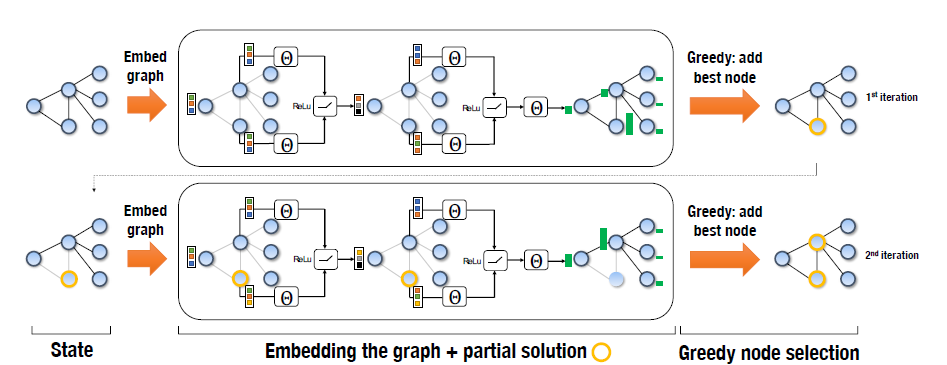
\includegraphics[scale=0.85]{images/graph-embedding.png}}
    \caption{Illustration of the graph embedding and greedy node selection framework proposed in Khalil et al. as applied to an instance of Minimum Vertex Cover. Figure adapted from \cite{khalil2017learning}}
    \label{fig:graph-embedding}
\end{figure*}

One of the first approaches to solve the COPs using unsupervised deep learning over the graph was proposed by \cite{khalil2017learning}. At this point, we have already referenced this work multiple times and we have also already discussed some drawbacks and extensions to this approach. Since it is such a seminal work, we discuss this approach in detail now. We compare their approach and result in the works that preceded them. For the most part, we have already compared this approach with other similar approaches such as \cite{li2018combinatorial} and \cite{mittal2019learning}.

\cite{khalil2017learning} proposed an end-to-end machine learning framework to solve COPs. They used deep graph embedding with reinforcement learning for automatically designing greedy heuristics. The learned policy behaved like a meta-algorithm that incrementally constructed a solution, with the action being determined by a graph embedding network over the current state of the solution. They exploited a common trait of real-world optimization problems | same optimization problem is solved again and again regularly, maintaining the same problem structure but differing in the data. Khalil et al. claimed that other approaches proposed before theirs \cite{vinyals2015pointer, bello2016neural} were generic and did not reflect the combinatorial structure of graph problems effectively. Besides, these approaches required a huge number of instances to learn to generalize to new ones. \cite{bello2016neural} used policy gradient for training which is not particularly sample-efficient \cite{khalil2017learning}. 

They adopted a greedy meta-algorithm design, whereby a feasible solution was constructed by the successive addition of nodes based on the graph structure and was maintained to satisfy the problem's graph constraints. For their graph embedding network, they used structure2vec \cite{dai2016discriminative} to represent the policy in the greedy algorithm. This deep learning architecture factorizes the nodes in the graph, capturing the properties of a node in the context of its graph neighborhood. This allows the policy to discriminate among nodes based on their usefulness and generalizes to problem instances of different sizes. They asserted that the prior works \cite{vinyals2015pointer, bello2016neural} used graph-agnostic sequence-to-sequence \cite{bahdanau2014neural} mapping that did not fully exploit graph structure. 

They used fitted Q-learning to learn a greedy policy that was parametrized by the graph embedding network. Their framework allowed the policy to optimize the objective function of the original problem instance directly. The main advantage of this approach is that it can deal with delayed rewards in a data-efficient way. Here, by delayed rewards, they meant the remaining increase in objective function value obtained by the greedy algorithm. In contrast, \cite{bello2016neural} which used the policy gradient approach updated the model parameters only once for the whole solution. This process of graph embedding and greedy approach to add the best node to a partial solution is shown in Figure \ref{fig:graph-embedding}. It shows two iterations of the graph embedding to an instance of Minimum Vertex Cover. 

The graph embedding network (structure2vec) defined the network architecture recursively according to an input graph structure. Node specific tags or features were aggregated recursively according to the graph's topology. After a few steps, the network produced a new embedding for each node, taking into account both graph characteristics and long-range interactions between these node features. The parameters of the network were trained end-to-end using Q-learning. Off-policy reinforcement learning such as Q-learning can be more sample efficient than their policy gradient counterparts \cite{gu2016q}. They claimed that this was because policy gradient methods require on-policy samples for the new policy obtained after each parameter update of the function approximator.

They trained their model (S2V-DQN) on three problems: MVC, MAXCUT, and TSP. They compared their method with \cite{bello2016neural} (PN-AC) which did not make full use of graph structure. Their result showed that the PN-AC algorithm performed well on TSP as graph structure is not as important in a fully connected TSP problem. However, in MVC and MAXCUT, where graph information is crucial, their approach performed significantly better than PN-AC. In real-world instances, their model significantly outperformed all competing methods for MVC, MAXCUT, and TSP. 

They made some important discoveries while examining the algorithms learned by S2V-DQN. For example, they noticed that S2V-DQN discovered an algorithm for MVC where nodes were selected to balance between their degrees and the connectivity of the remaining graph. Based on such results, they suggested that S2V-DQN may also be a good assistive tool for discovering new algorithms for lesser-known graph optimization problems.    

The most recent work that exploits the structure of the problems defined over a graph is done by Barrett et al. \cite{barrett2019exploratory}. Barrett et al. claim that learning a policy that directly produces a single, optimal solution is often impractical because of the complexity of many combinatorial problems. Therefore, they propose an exploratory combinatorial optimization (ECO-DQN) in which an agent seeks to continuously improve the solution by learning to explore at test time. This is different than S2V-DQN and approaches following it which incrementally construct solutions one element at a time as described in \cite{khalil2017learning}.  

\section{Challenges}
Despite promising results shown by deep learning methodologies to solving COPs, there are still multiple challenges. A lot of these challenges are mostly because of the nature of the problems themselves, most of which are NP-hard. \cite{bengio2018machine} discuss some of these persistent challenges in this field.

First, finding a feasible solution to COPs is not so trivial. \cite{bengio2018machine} claim that algorithms learned by deep learning methodologies do not give any guarantee in terms of optimality or feasibility. This is because the algorithm is learning a heuristic rather than learning the solution. Like any heuristic algorithm, there is always a risk of not reaching a close enough optimal solution or even feasible solutions. Bengio et al. suggest that because neural networks are so complex, they should be designed in such as way that they do not break the differentiability of COPs, to make sure that network can generate feasible solutions.

Second, scaling the proposed methodologies to solve larger instances of COPs is still a challenging task. Even though some recent works are dealing with this issue, there has not been a promising result. If a model trained on instances up to a certain size COP is evaluated on larger instances, the challenge exists in terms of generalization \cite{bengio2018machine}. Previous works to solve TSP using deep learning, while attempting to solve larger instances, observe degrading performance as size increases much beyond the sizes seen during training \cite{vinyals2015pointer, bello2016neural, khalil2017learning}. Training on larger sized instances can also be computationally expensive.

Finally, even though previous work has been successful in generalizing their approach to different well-studied COPs such as Knapsack and TSP \cite{bello2016neural}, it is still a challenging task to generalize such approaches on lesser-known COPs. Smith-Miles and Bowly \cite{smith2015generating} asserted that often, a new algorithm is claimed to be superior by showing that it outperforms a state-of-the-art approach on a set of well-studied instances.  

% Finally, it is also hard to generate data for some COPs. For the application that we are well aware of, it is not very hard to collect data. However, if we are not very familiar with a COP and do not have much historical data, it is a challenge to train a policy to find a solution to such problems. To address this issue, \cite{bengio2018machine} suggests generalizing such problems to a known family of instances. Even so, \cite{bengio2018machine} hints that it is hard to generate problems that capture the essence of real applications because these COPs are high dimensional, highly structured, and troublesome to visualize. 

\section{Discussion and Summary}
Despite all these challenges, we believe that deep learning has a lot of potential in the domain of solving NP-hard COPs. Some recent works have shown promising results, especially because of the use of DRL. For example, \cite{mittal2019learning} designed a deep reinforcement learning model called GCOMB and trained on billion-sized graphs, showing some promising results in dealing with the scalability issue. Barrett et al. \cite{barrett2019exploratory} designed an exploratory combinatorial optimization using deep Q-learning (ECO-DQN) to train an agent and continually improved the solution by learning to explore at test time. Most of the previous deep learning methodologies constructed the solution subset incrementally, adding one element at a time \cite{khalil2017learning, li2018combinatorial}. However, the irreversible nature of these approaches prevents the agent from revising its earlier decisions. Given the complexity of the problem, it may be necessary to revisit the earlier decisions, which is addressed using ECO-DQN \cite{barrett2019exploratory}.


In this paper, we surveyed some prominent work proposed to solve COPs using deep learning methodologies. We briefly discussed some exact and approximate algorithms to solve such a problem. However, because most of these problems are NP-hard, such exact and heuristic-based algorithms are not feasible for large-sized COPs. This led researchers to look into machine learning to let the algorithm figure out the essential heuristic to find the optimal solutions. We discussed some pioneer works based on Hopfield neural network \cite{hopfield1985neural} and Self-Organizing Maps based approaches \cite{kohonen1982self}. Even though the field looked promising, some major setbacks drove researchers away from this field after the turn of $21^{st}$ century. 

With the advent of deep learning, researchers started using artificial neural networks once again to tackle this problem with promising results. Researchers have used both supervised and unsupervised learning approaches to find the optimal solution to COPs. Some of the prominent supervised learning approaches include \cite{vinyals2015pointer} and \cite{khalil2017learning}. Vinyals et al. used Pointer Networks which is based on sequence-to-sequence learning with attention mechanism whereas Li et al. used Graph Convolutional Network (GCN). The field of unsupervised learning to solve COPs has been heavily influenced by DRL based approaches such as Deep Q-Learning (DQN). Some of the prominent works are \cite{bello2016neural} who extended Pointer Networks with the policy gradient algorithm and \cite{khalil2017learning} who used graph embedding network with Q-learning. We also presented some challenges in this field at the moment, which includes a lack of scalability, feasibility, and methods to generate training data. Finally, in light of some promising recent work being done to tackle some of these problems using deep reinforcement learning, we recommend the research community to focus more on DRL methodologies to solving COPs. 

\section*{Acknowledgment}
We would like to thank Dr. Benjamin Mitchell for giving us helpful guidance and impetus to start this project. The authors would also like to thank Subash Nepal for crucial guidance in the process of writing and structuring the paper.


% we can use newpage to force the bibliography to start at the top of its own
% page (or column, in a 2-column format)
\newpage

% many different styles of bibliography are available; here we specify the
% bib-style provided for ICML 2018
\bibliographystyle{icml2018}

% the bibliography command should contain the name of your .bib file, minus the
% extension.
\bibliography{references}

\end{document}
% because "document" is an environment, you need to have a closing tag at the
% end of your document.  Anything written after this tag will not be included in
% the generated output.
For example, here is some text that will never show up.
